% 第8章第6节：Hamilton系统与保结构计算（Hamilton方程与守恒结构；辛Euler、Leapfrog与长期误差）。

\section{Hamilton系统与保结构计算}
\label{sec:ode-hamiltonian}

前面的稳定性分析多半依赖耗散：能量或某个Lyapunov函数沿轨迹下降，轨迹最终停下。无摩擦的摆、行星的轨道、分子中原子的振动却不耗散，它们长时间运动而不停下。这类系统的特殊结构既决定了精确解的性质，也对数值方法提出了上一节没有考虑的要求。本节把位置与动量一起作为状态，在欧氏坐标与矩阵形式下研究这种结构；一般流形上的辛几何可参考\BookChapterRef{chap:differential-geometry-and-symmetry}{卷四“非线性空间与流形”章}。

\subsection{Hamilton方程与守恒结构}
\label{sec:ode-hamilton-equations}

\paragraph{从能量写出运动方程}
位置相同而速度不同的物体有不同的未来，所以力学状态要同时记录位置$\bm q\in\mathbb R^d$与动量$\bm p\in\mathbb R^d$。设质量矩阵$\bm M$对称正定，势能$U(\bm q)$连续可微，总能量为动能加势能：
\begin{equation}
  H(\bm q,\bm p)=U(\bm q)+\frac12\bm p^\top\bm M^{-1}\bm p.
  \label{eq:ode-separable-hamiltonian}
\end{equation}
运动方程是：位置的变化率等于速度$\bm M^{-1}\bm p$，动量的变化率等于力$-\nabla U(\bm q)$。对照$H$的偏导数，这恰好是
\begin{equation}
  \dot{\bm q}=\nabla_{\bm p}H,\qquad\dot{\bm p}=-\nabla_{\bm q}H.
  \label{eq:ode-hamilton-equations}
\end{equation}
一个标量函数通过“对动量求导给出位置的变化、对位置求导取负号给出动量的变化”组织出一对方程。摆取$M=1$，$H=p^2/2+1-\cos q$，式~\eqref{eq:ode-hamilton-equations}给出$\dot q=p$、$\dot p=-\sin q$；谐振子取$H=(q^2+p^2)/2$，得$\dot q=p$、$\dot p=-q$。

把$\bm q,\bm p$合成$\bm z=(\bm q^\top,\bm p^\top)^\top\in\mathbb R^{2d}$，方程可以写成一个式子。

\begin{definition}[Hamilton系统]
  \label{def:ode-hamiltonian-system}
  设$H:\mathbb R^{2d}\to\mathbb R$二阶连续可微，令
  \[
    \bm J=\begin{bmatrix}\bm0&\bm I_d\\-\bm I_d&\bm0\end{bmatrix}.
  \]
  方程$\dot{\bm z}=\bm J\nabla H(\bm z)$称为以$H$为\term{Hamilton量}的\term{Hamilton系统}。$H$具有形式~\eqref{eq:ode-separable-hamiltonian}时称为可分的。
\end{definition}

$\bm J$是反对称矩阵，$\bm J^\top=-\bm J$，并且$\bm J^2=-\bm I$。它把梯度转动成运动方向：在$d=1$时，$\bm J\nabla H=(\partial_pH,-\partial_qH)$正是把梯度$(\partial_qH,\partial_pH)$顺时针转了九十度。

\paragraph{同一能量的两种流}
同一个函数$H$可以产生完全不同的动力学。梯度流$\dot{\bm z}=-\nabla H$沿最陡的方向下降；Hamilton流$\dot{\bm z}=\bm J\nabla H$沿与梯度垂直的方向运动。图~\ref{fig:ode-hamilton-gradient-flow}取$H=(q^2+p^2)/2$并从同一点出发：Hamilton流沿圆周永远转下去，梯度流径直落向原点。

\begin{figure}[htbp]
  \centering
  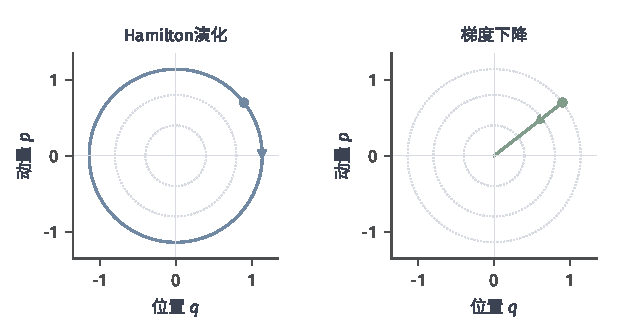
\includegraphics[width=107mm]{figures/00-shared/mathematical-preliminaries-lower/02-dynamical-systems-control-decision-and-games/matplotlib/reader-hamilton-gradient-flow/figure.pdf}
  \caption{同一函数$H(q,p)=(q^2+p^2)/2$下的两种精确流。两面板均从$(q_0,p_0)=(0.9,0.7)$出发，绘制$0\leq t\leq2\pi$；灰色虚线是相同的能量等值线，箭头表示运动方向。左侧Hamilton系统$\dot q=p,\dot p=-q$保持能量，右侧梯度流$\dot q=-q,\dot p=-p$使能量下降。}
  \label{fig:ode-hamilton-gradient-flow}
\end{figure}

两者沿轨迹的能量变化分别是
\[
  \frac{\mathrm d}{\mathrm dt}H=\nabla H^\top\bm J\nabla H=0,\qquad
  \frac{\mathrm d}{\mathrm dt}H=-\nabla H^\top\nabla H=-\|\nabla H\|_2^2,
\]
第一个等式成立是因为反对称矩阵的二次型为零。更一般地，取对称半正定矩阵$\bm R$，方程$\dot{\bm z}=(\bm J-\bm R)\nabla H$满足$\dot H=-\nabla H^\top\bm R\nabla H\leq0$。阻尼摆正是$\bm R=\operatorname{diag}(0,c)$的情形，能量导数为$-cp^2$，这就是第~\ref{sec:ode-lyapunov}小节用过的计算。能量函数相同，动力学由它前面的矩阵决定：反对称部分产生守恒的旋转，对称半正定部分产生耗散。梯度流用于优化，在第~\ref{chap:opt-smooth}章作为离散算法的连续对照出现；Hamilton流则描述保守运动。

\paragraph{能量守恒}
上面对谐振子的计算只用到了$\bm J$的反对称性，并不依赖$H$的具体形式。把它写成一般结论：

\begin{theorem}[Hamilton系统的能量守恒]
  \label{thm:ode-energy-conservation}
  设$H$连续可微，$\bm z(t)$是Hamilton系统在某区间上的解，则$H(\bm z(t))$在该区间上为常数。
\end{theorem}

\begin{proof}
  链式法则给出$\frac{\mathrm d}{\mathrm dt}H(\bm z(t))=\nabla H^\top\dot{\bm z}=\nabla H^\top\bm J\nabla H=0$。
\end{proof}

因此轨迹被限制在初始能量的等值面上。若这些等值面有界（例如势能$U$在无穷远处趋于无穷），轨迹就留在紧集中，由定理~\ref{thm:ode-escape}对全部时间存在。守恒本身并不保证有界：自由粒子$H=p^2/2$保持能量，但$p\neq0$时$q(t)=q_0+pt$无界。若$H$显含时间，同样的计算只给出$\frac{\mathrm d}{\mathrm dt}H=\partial_tH$，能量不再守恒。

\paragraph{辛结构与相空间体积}
能量守恒是对一条轨迹的标量约束，它没有说明一团相邻的初态怎样变形。第~\ref{sec:ode-flows}小节已经看到，无阻尼摆的流把圆盘拉长弯曲，面积却保持不变。现在说明这背后的结构。

取相空间中两个小位移$\bm u,\bm v\in\mathbb R^{2d}$。在$d=1$时，它们张成的平行四边形的有向面积是$u_qv_p-u_pv_q=\bm u^\top\bm J\bm v$。$d>1$时，$\bm u^\top\bm J\bm v=\sum_{i=1}^d(u_{q_i}v_{p_i}-u_{p_i}v_{q_i})$是每一对“位置—动量”坐标平面上有向面积之和。

\begin{definition}[辛形式与辛映射]
  \label{def:ode-symplectic-map}
  对$\bm u,\bm v\in\mathbb R^{2d}$，称$\omega(\bm u,\bm v)=\bm u^\top\bm J\bm v$为标准\term{辛形式}。开集上的连续可微映射$\bm\psi$若在每一点的Jacobian矩阵$\bm G=\partial\bm\psi$都满足
  \begin{equation}
    \bm G^\top\bm J\bm G=\bm J,
    \label{eq:ode-symplectic-condition}
  \end{equation}
  称为\term{辛映射}（symplectic map）。
\end{definition}

条件~\eqref{eq:ode-symplectic-condition}说，任意两个小位移经映射的线性部分作用后，辛形式的值不变。取行列式得$(\det\bm G)^2=1$，所以辛映射保持体积（再由连续性可知行列式为$1$，也保持定向）。反过来不成立：在坐标$(q_1,q_2,p_1,p_2)$下，$\bm G=\operatorname{diag}(2,1,1,\tfrac12)$的行列式为$1$，保持体积，却把第一对坐标平面上的面积乘以$2$、第二对乘以$\tfrac12$，不满足式~\eqref{eq:ode-symplectic-condition}。总体积允许不同坐标对之间相互抵消，辛性不允许。$d=1$时二者等价，辛就是保面积。

\begin{theorem}[Hamilton流是辛映射]
  \label{thm:ode-hamiltonian-flow-symplectic}
  设$H$二阶连续可微，$\bm\varphi_t$是Hamilton系统的流。则在其定义域上，每个$\bm\varphi_t$都是辛映射，并且$\det\partial\bm\varphi_t=1$。
\end{theorem}

\begin{proof}
  由定理~\ref{thm:ode-variational-equation}，$\bm G_t=\partial\bm\varphi_t(\bm z_0)$满足变分方程$\dot{\bm G}_t=\bm J\bm S\bm G_t$，$\bm G_0=\bm I$，其中$\bm S=\nabla^2H(\bm z(t))$是对称的Hessian矩阵。于是
  \[
    \begin{aligned}
    \frac{\mathrm d}{\mathrm dt}\bigl(\bm G_t^\top\bm J\bm G_t\bigr)&=\bm G_t^\top\bigl((\bm J\bm S)^\top\bm J+\bm J\bm J\bm S\bigr)\bm G_t\\
    &=\bm G_t^\top\bigl(\bm S\bm J^\top\bm J+\bm J^2\bm S\bigr)\bm G_t=\bm G_t^\top(\bm S-\bm S)\bm G_t=\bm0,
    \end{aligned}
  \]
  这里用了$\bm J^\top\bm J=\bm I$与$\bm J^2=-\bm I$。初值$\bm G_0^\top\bm J\bm G_0=\bm J$，所以$\bm G_t^\top\bm J\bm G_t=\bm J$。行列式的结论可由定理~\ref{thm:ode-state-transition-properties}的Liouville公式直接得到：$\operatorname{tr}(\bm J\bm S)=\operatorname{tr}(\bm S\bm J^\top)=-\operatorname{tr}(\bm J\bm S)$，故迹为零，$\det\bm G_t=e^0=1$。
\end{proof}

这解释了图~\ref{fig:ode-flow-deformation}：无阻尼摆的流保持面积，阻尼使向量场的迹变为$-c$，面积按$e^{-ct}$缩小。三种性质需要分开：能量守恒是沿一条轨迹的标量性质；体积保持是对一团初值的整体性质；辛性比体积保持更强，约束每一对坐标平面。它们互不蕴含。保持能量而不保持面积的例子是：在谐振子的相平面上用极坐标$(r,\theta)$，令$\bm\psi(r,\theta)=(r,\theta+\epsilon\sin\theta)$，$0<\epsilon<1$。它把每个能量圆映到自身，因而保持$H=r^2/2$；但它沿圆周方向的伸缩率是$1+\epsilon\cos\theta$，不是常数，面积不保持。

\subsection{辛Euler、Leapfrog与长期误差}
\label{sec:ode-symplectic-integrators}

\paragraph{显式Euler为何让能量漂移}
把显式Euler用于谐振子$\dot q=p$，$\dot p=-q$，一步更新为
\[
  \begin{bmatrix}q_{n+1}\\p_{n+1}\end{bmatrix}=\begin{bmatrix}1&h\\-h&1\end{bmatrix}\begin{bmatrix}q_n\\p_n\end{bmatrix},
  \qquad q_{n+1}^2+p_{n+1}^2=(1+h^2)(q_n^2+p_n^2).
\]
每一步能量都精确地乘以$1+h^2$，轨迹沿螺线向外。$h=0.1$时，$120$步后能量变为原来的$1.01^{120}\approx3.30$倍，见图~\ref{fig:ode-symplectic-energy}(a)。后向Euler的因子是$1/(1+h^2)$，轨迹向内螺旋。从稳定域的角度看，谐振子的特征值$\pm\mathrm i$乘以$h$落在虚轴上。显式Euler的稳定域只在原点处碰到虚轴，$|1+\mathrm ih|=\sqrt{1+h^2}>1$；后向Euler在虚轴上（原点除外）满足$|1/(1-\mathrm ih)|<1$。精确流的$|e^{\mathrm ih}|=1$恰好介于二者之间，任何偏向一侧的误差都会在长时间里单调积累。

RK4的稳定域包含虚轴上的一段，在那里$|R_{\mathrm{RK4}}(\mathrm iy)|^2=1-y^6/72+y^8/576$，对$0<|y|\leq2\sqrt2$略小于$1$。所以RK4用于谐振子时能量也单调地减小，只是每步的损失是$O(h^6)$，很慢。问题不在于阶数不够高，而在于方法没有尊重系统的结构。

\paragraph{辛Euler与Leapfrog}
对可分的Hamilton量，可以把一步拆成两种可以精确求解的子运动。只保留势能时，$\dot{\bm q}=\bm0$，$\dot{\bm p}=-\nabla U(\bm q)$，位置不动，动量受一次“冲击”：$(\bm q,\bm p)\mapsto(\bm q,\bm p-c\nabla U(\bm q))$，记为$\bm\Phi_U^c$。只保留动能时，$\dot{\bm q}=\bm M^{-1}\bm p$，$\dot{\bm p}=\bm0$，动量不变，位置“漂移”：$(\bm q,\bm p)\mapsto(\bm q+c\bm M^{-1}\bm p,\bm p)$，记为$\bm\Phi_K^c$。两者都是对应子系统的精确流。

先冲击、再漂移，得到\term{辛Euler法}：
\begin{equation}
  \bm p_{n+1}=\bm p_n-h\nabla U(\bm q_n),\qquad\bm q_{n+1}=\bm q_n+h\bm M^{-1}\bm p_{n+1}.
  \label{eq:ode-symplectic-euler}
\end{equation}
与显式Euler的唯一区别是：位置更新使用已经更新过的动量。把冲击对半分开、夹住一次整步漂移，得到对称的\term{Leapfrog方法}（也称蛙跳法或Störmer--Verlet方法）：
\begin{equation}
  \begin{aligned}
  \bm p_{n+1/2}&=\bm p_n-\frac h2\nabla U(\bm q_n),\\
  \bm q_{n+1}&=\bm q_n+h\bm M^{-1}\bm p_{n+1/2},\\
  \bm p_{n+1}&=\bm p_{n+1/2}-\frac h2\nabla U(\bm q_{n+1}).
  \end{aligned}
  \label{eq:ode-leapfrog}
\end{equation}
即$\bm\Psi_h=\bm\Phi_U^{h/2}\circ\bm\Phi_K^h\circ\bm\Phi_U^{h/2}$。连续两步之间，后一步开头的半步冲击与前一步结尾的半步冲击使用同一个力$\nabla U(\bm q_{n+1})$，所以每步只需计算一次力。辛Euler是一阶方法，Leapfrog是二阶方法。

用于谐振子（$U=q^2/2$，$M=1$），两者的更新矩阵分别是
\[
  \begin{bmatrix}1-h^2&h\\-h&1\end{bmatrix},\qquad
  \begin{bmatrix}1-h^2/2&h\\-h+h^3/4&1-h^2/2\end{bmatrix},
\]
行列式都是$1$。图~\ref{fig:ode-symplectic-energy}(a)中，两者在$120$步内都紧贴单位圆，没有向外或向内的漂移。

\begin{figure*}[htbp]
  \centering
  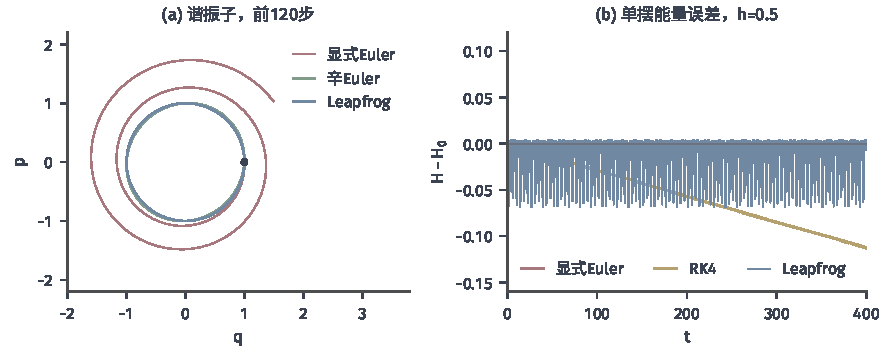
\includegraphics[width=150mm]{figures/03-optimization-evolution-and-signals/02-processes-and-trajectory-evolution/matplotlib/ode-symplectic-energy/figure.pdf}
  \caption{保守系统的长期数值行为。(a)谐振子$\dot q=p$，$\dot p=-q$，从$(1,0)$出发，步长$h=0.1$，各算$120$步：显式Euler（红）的能量按$1.01^n$增长，$120$步后为初值的约$3.30$倍；辛Euler（绿）与Leapfrog（蓝）贴近灰色虚线所示的精确圆周。(b)单摆$\dot q=p$，$\dot p=-\sin q$，从$(2,0)$出发（$H_0=1-\cos2\approx1.416$），步长$h=0.5$，计算到$t=400$，纵轴为能量误差$H-H_0$：显式Euler在约$t=3$时误差即超出图示范围；RK4（黄）单调下降到约$-0.113$；Leapfrog（蓝）在$[-0.069,0.004]$内振荡而不漂移。}
  \label{fig:ode-symplectic-energy}
\end{figure*}

\paragraph{验证保辛与可逆}
设$U$二阶连续可微。冲击与漂移的Jacobian矩阵为
\[
  \bm G_U=\begin{bmatrix}\bm I&\bm0\\-c\nabla^2U&\bm I\end{bmatrix},\qquad
  \bm G_K=\begin{bmatrix}\bm I&c\bm M^{-1}\\\bm0&\bm I\end{bmatrix}.
\]
直接相乘可验证$\bm G_U^\top\bm J\bm G_U=\bm J$：计算中出现的是$-c\nabla^2U+c(\nabla^2U)^\top$，由Hessian矩阵的对称性为零；同理$\bm M^{-1}$的对称性给出$\bm G_K^\top\bm J\bm G_K=\bm J$。辛映射的复合仍是辛映射，因为$(\bm G_1\bm G_2)^\top\bm J(\bm G_1\bm G_2)=\bm G_2^\top(\bm G_1^\top\bm J\bm G_1)\bm G_2=\bm G_2^\top\bm J\bm G_2=\bm J$。所以辛Euler与Leapfrog都是辛映射。这也说明了它们为何与显式Euler不同：显式Euler同时用旧的位置和旧的动量更新两者，用于谐振子时Jacobian的行列式是$1+h^2$，不是辛映射。

Leapfrog还有一个对称性。每个子步把$c$换成$-c$就得到它的逆，而三个子步对称排列，所以$\bm\Psi_h^{-1}=\bm\Psi_{-h}$：向后走一步等于把步长取负。若$\bm R(\bm q,\bm p)=(\bm q,-\bm p)$表示动量反向，还有$\bm R\circ\bm\Psi_h\circ\bm R=\bm\Psi_h^{-1}$：把动量反过来走一步，再把动量反回来，恰好回到出发前的状态。这就是数值上的时间可逆性，与精确流的可逆性相对应。辛Euler没有这种对称性，它的逆是“先漂移、后冲击”的另一种排列。

\paragraph{保辛不等于精确保能量}
辛方法并不精确保持$H$。对谐振子的Leapfrog，更新矩阵的迹为$2-h^2$，行列式为$1$；当$0<h<2$时，两个特征值是单位圆上一对不同的共轭复数，可以直接验证它精确保持修正的二次型
\[
  \widetilde H_h(q,p)=\Bigl(1-\frac{h^2}4\Bigr)q^2+p^2.
\]
这是一族椭圆而不是原来的能量圆。例如从$(1,0)$出发取$h=1$，一步得到$(\tfrac12,-\tfrac34)$，原能量从$\tfrac12$变成$\tfrac{13}{32}$，修正二次型却保持为$\tfrac34$。原能量在椭圆上周期性地变化，偏差是$O(h^2)$，但不会单调地漂移。辛Euler类似地保持$q^2+p^2-hqp$。$h>2$时Leapfrog的更新矩阵有模大于$1$的特征值，数值解指数增长；保辛并不意味着任意步长都稳定。

非线性情形没有这样简单的修正二次型。图~\ref{fig:ode-symplectic-energy}(b)取单摆与较大的步长$h=0.5$计算到$t=400$：Leapfrog的能量误差始终在$[-0.069,0.004]$内振荡；RK4每步的局部误差小得多，能量却单调下降，到$t=400$约少了$0.113$；显式Euler的能量误差在$t\approx3$时就超出了图示范围。还要注意，RK4每步调用$4$次向量场，Leapfrog只需$1$次力的计算。对一般光滑的Hamilton量，辛方法在长时间内能量误差有界的表现，依赖步长足够小、$H$足够光滑以及轨道留在有界区域等条件，相应的理论（后向误差分析）超出本书范围。

\paragraph{用于采样时还缺什么}
Leapfrog的保体积与可逆性，使它成为Hamilton Monte Carlo采样中的标准积分器\scite{pgm-sampling-neal2011}。但它不能单独完成采样。精确的Hamilton流保持能量，只在一个能量等值面上运动，无法探索不同能量的状态，所以需要定期从相应分布中重新抽取动量。Leapfrog又只近似保持能量，若不加修正，所得样本的分布会有偏差，所以每条数值轨迹的终点还要按能量误差决定是否接受。保辛、可逆和保体积使这个接受概率可以简单地计算，但并不能代替它。完整的构造与正确性证明属于随机过程，在第~\ref{chap:discrete-time-stochastic-processes}章讨论。
